\chapter{Resultados Parcias}\label{cap:resultados-parcias}

Serão aqui apresentados os resultados alcançados até o momento da produção da proposta.


\section{Levantamento de requisitos e priorização}

O levantamento de requisitos constituiu a primeira etapa do trabalho. Os requisitos foram identificados principalmente a partir das observações da orientadora Dra. Sediane Carmem Lunardi Hernandes, que apontou, no sistema E-Museu, a necessidade de aprimoramentos na estrutura do código, bem como a ausência de testes automatizados, evidenciando a demanda por refatoração e pelo desenvolvimento de novas funcionalidades.

Após discussões e alinhamentos, os requisitos receberam ajustes a partir das contribuições do coorientador Dr. Diego Marczal e dos professores Me. Dênis Lucas Silva e Dr. Emerson André Fedechen, especialmente durante a primeira banca, o que permitiu um refinamento mais preciso e alinhado aos objetivos centrais do trabalho.

Com os requisitos definidos, foi aplicada a técnica de priorização MoSCoW, com o objetivo de direcionar o desenvolvimento para as funcionalidades de maior impacto no sistema, otimizando o uso do tempo, esforço e recursos disponíveis. O resultado dessa priorização é apresentado na Figura 2.

\begin{figure}[H]
    \centering
    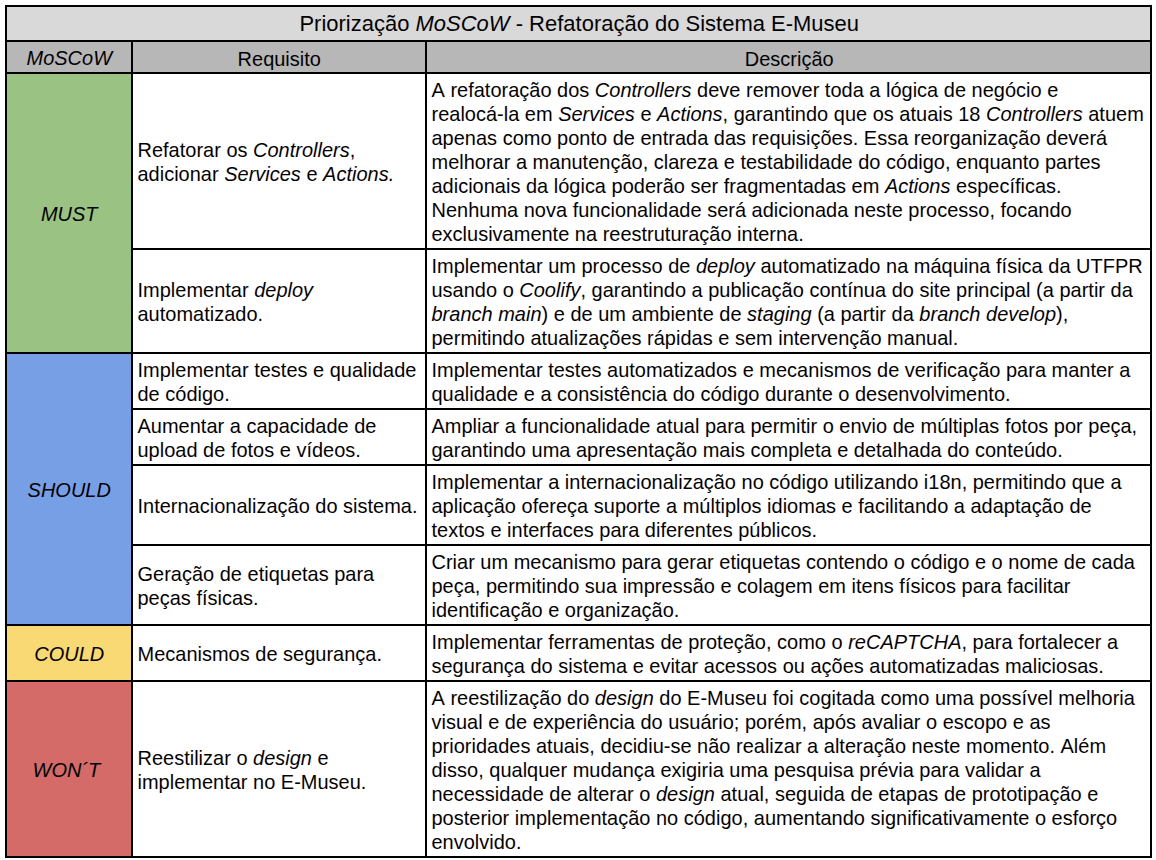
\includegraphics[width=\textwidth]{figuras/moscow.png}
    \caption{Priorização \acrshort{moscow}.}
    \label{fig:moscow}
    \caption*{\textbf{Fonte:} Autoria própria.}
\end{figure}



\subsection{Elaboração da Documentação do Gitflow}

Para garantir um fluxo de desenvolvimento consistente e devidamente documentado, foi realizada, previamente ao início da implementação, uma elaboração completa da documentação referente ao Gitflow, convenções de \textit{commits}, gestão de \textit{issues} e demais práticas relacionadas ao versionamento. Toda essa documentação está disponível no repositório oficial do projeto \cite{gitflowdoc}.


\subsection{Criação do repositório do E-Museu e configuração de ambiente}

O repositório do E-Museu foi criado a partir de um \textit{fork}, que se trata de uma cópia independente de um projeto existente, permitindo sua evolução de forma separada da primeira versão desenvolvida por \cite{gonzaga2024}. A partir dele, estruturou-se uma configuração inicial de ambiente utilizando Docker Compose, servindo como base para o desenvolvimento posterior \cite{emuseurepo}.
